\section{Auswertung}
\subsection{Verifizierung der Funktionsweise des Lock-In-Verstärkers.}
Zuerst wird die Schaltung aus \autoref{fig:f3} aufgebaut und wie 
in der \autoref{sec:Theorie} beschrieben Die Spannungsamplitude in abhängigkeit der 
Phasenverschiebung $\phi$ betrachtet. Die Werte Der Spannungsamplitude in abhängigkeit 
von $\phi$ sind in \autoref{tab:10} aufgetragen und in \autoref{fig:10} graphisch dargestellt.
\begin{table}[H]
    \centering
    \caption{Meswerte Stromstärke pro phasenverschiebung}
    \label{tab:10}
    \begin{tblr}{
        colspec = {S S },
        row{1} = {guard, mode=math},}
           \toprule
            \text{Phase} \left(\unit{\degree}\right) & U \left(\unit{\volt}\right)\\
           \midrule
            30  &3\\
            60  &6\\
            90  &6\\
            120 &5.5\\
            150 &2\\
            180 &-0.5\\
            210 &-3\\
            240 &-5.5\\
            270 &-6\\
            300 &-5.5\\
            330 &-2\\
            630 &0\\
            \bottomrule
    \end{tblr}
\end{table}

%Plot Phase/Spannung
\begin{figure}[H]
    \caption{}
    \label{fig:10}
    \centering
    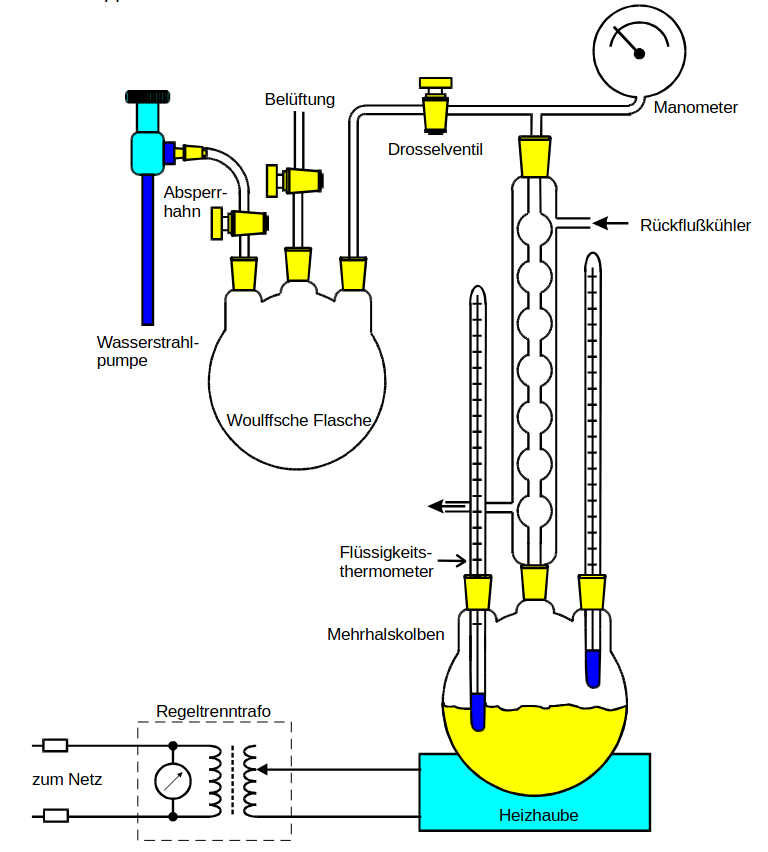
\includegraphics{"build/teil1.pdf"}
\end{figure}
Des weiteren Wurden die Werte aus \autoref{tab:10} in \autoref{fig:10} durch eine Funktion 
folgender Form geplottet.
\begin{equation}
    f\left(\phi\right) = a \cdot \sin \left(b \cdot \phi + c\right) + d
\end{equation}
Die ausgleichsrechnung mithilfe eines Curve Fits aus der Python Bibiliothek Scipy gibt 
die Ausgleichsparameter 
\begin{align*}
    a = & \qty{-6.1(0.4)}{\volt}   \\
    b = & \qty{1.00(0.04)}{}     \\
    c = & \qty{164(0.16)}{}    \\
    d = & \qty{0.00(0.31)}{\volt}      
\end{align*}

\begin{figure}
    \caption{Spannung bei 90$\unit{\degree}$}
    \label{fig:12}
    \centering
    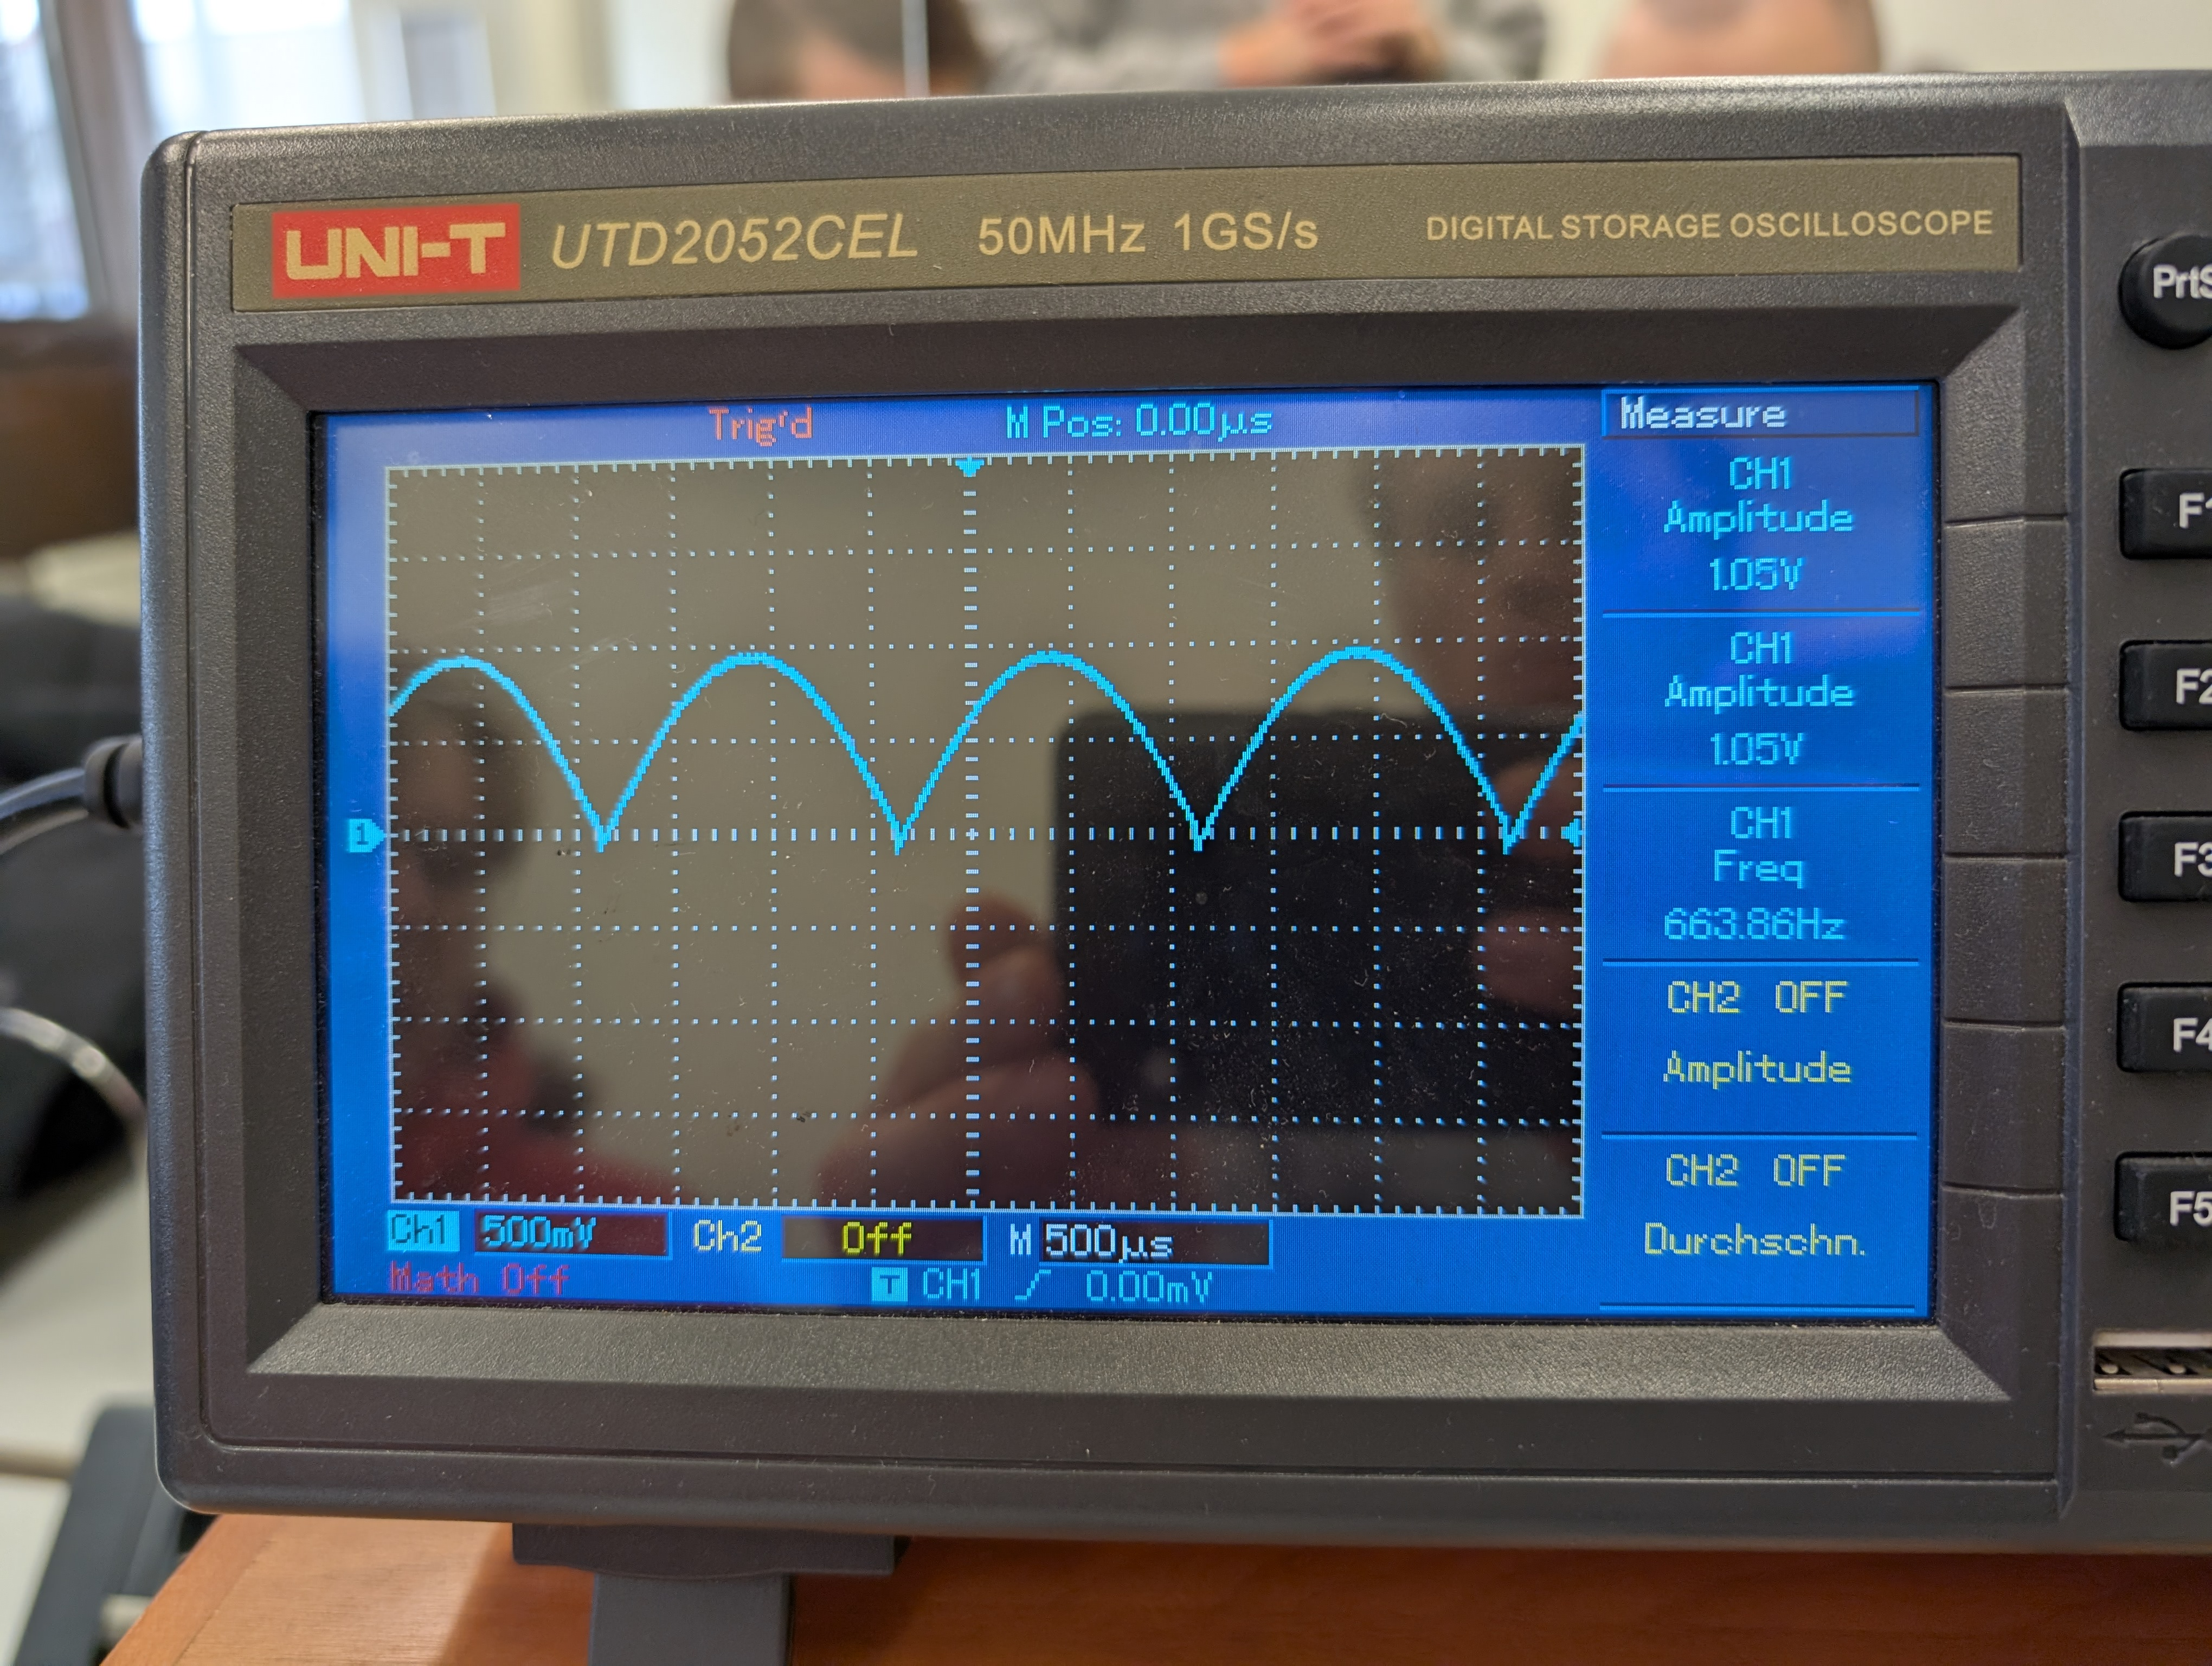
\includegraphics[width=0.5\textwidth]{"Bilder/90.jpg"}
\end{figure}
\begin{figure}
    \caption{Spannung bei 180$\unit{\degree}$}
    \label{fig:12}
    \centering
    \includegraphics[width=0.5\textwidth]{"Bilder/180.jpg"}
\end{figure}
\begin{figure}
    \caption{Spannung bei 270$\unit{\degree}$}
    \label{fig:12}
    \centering
    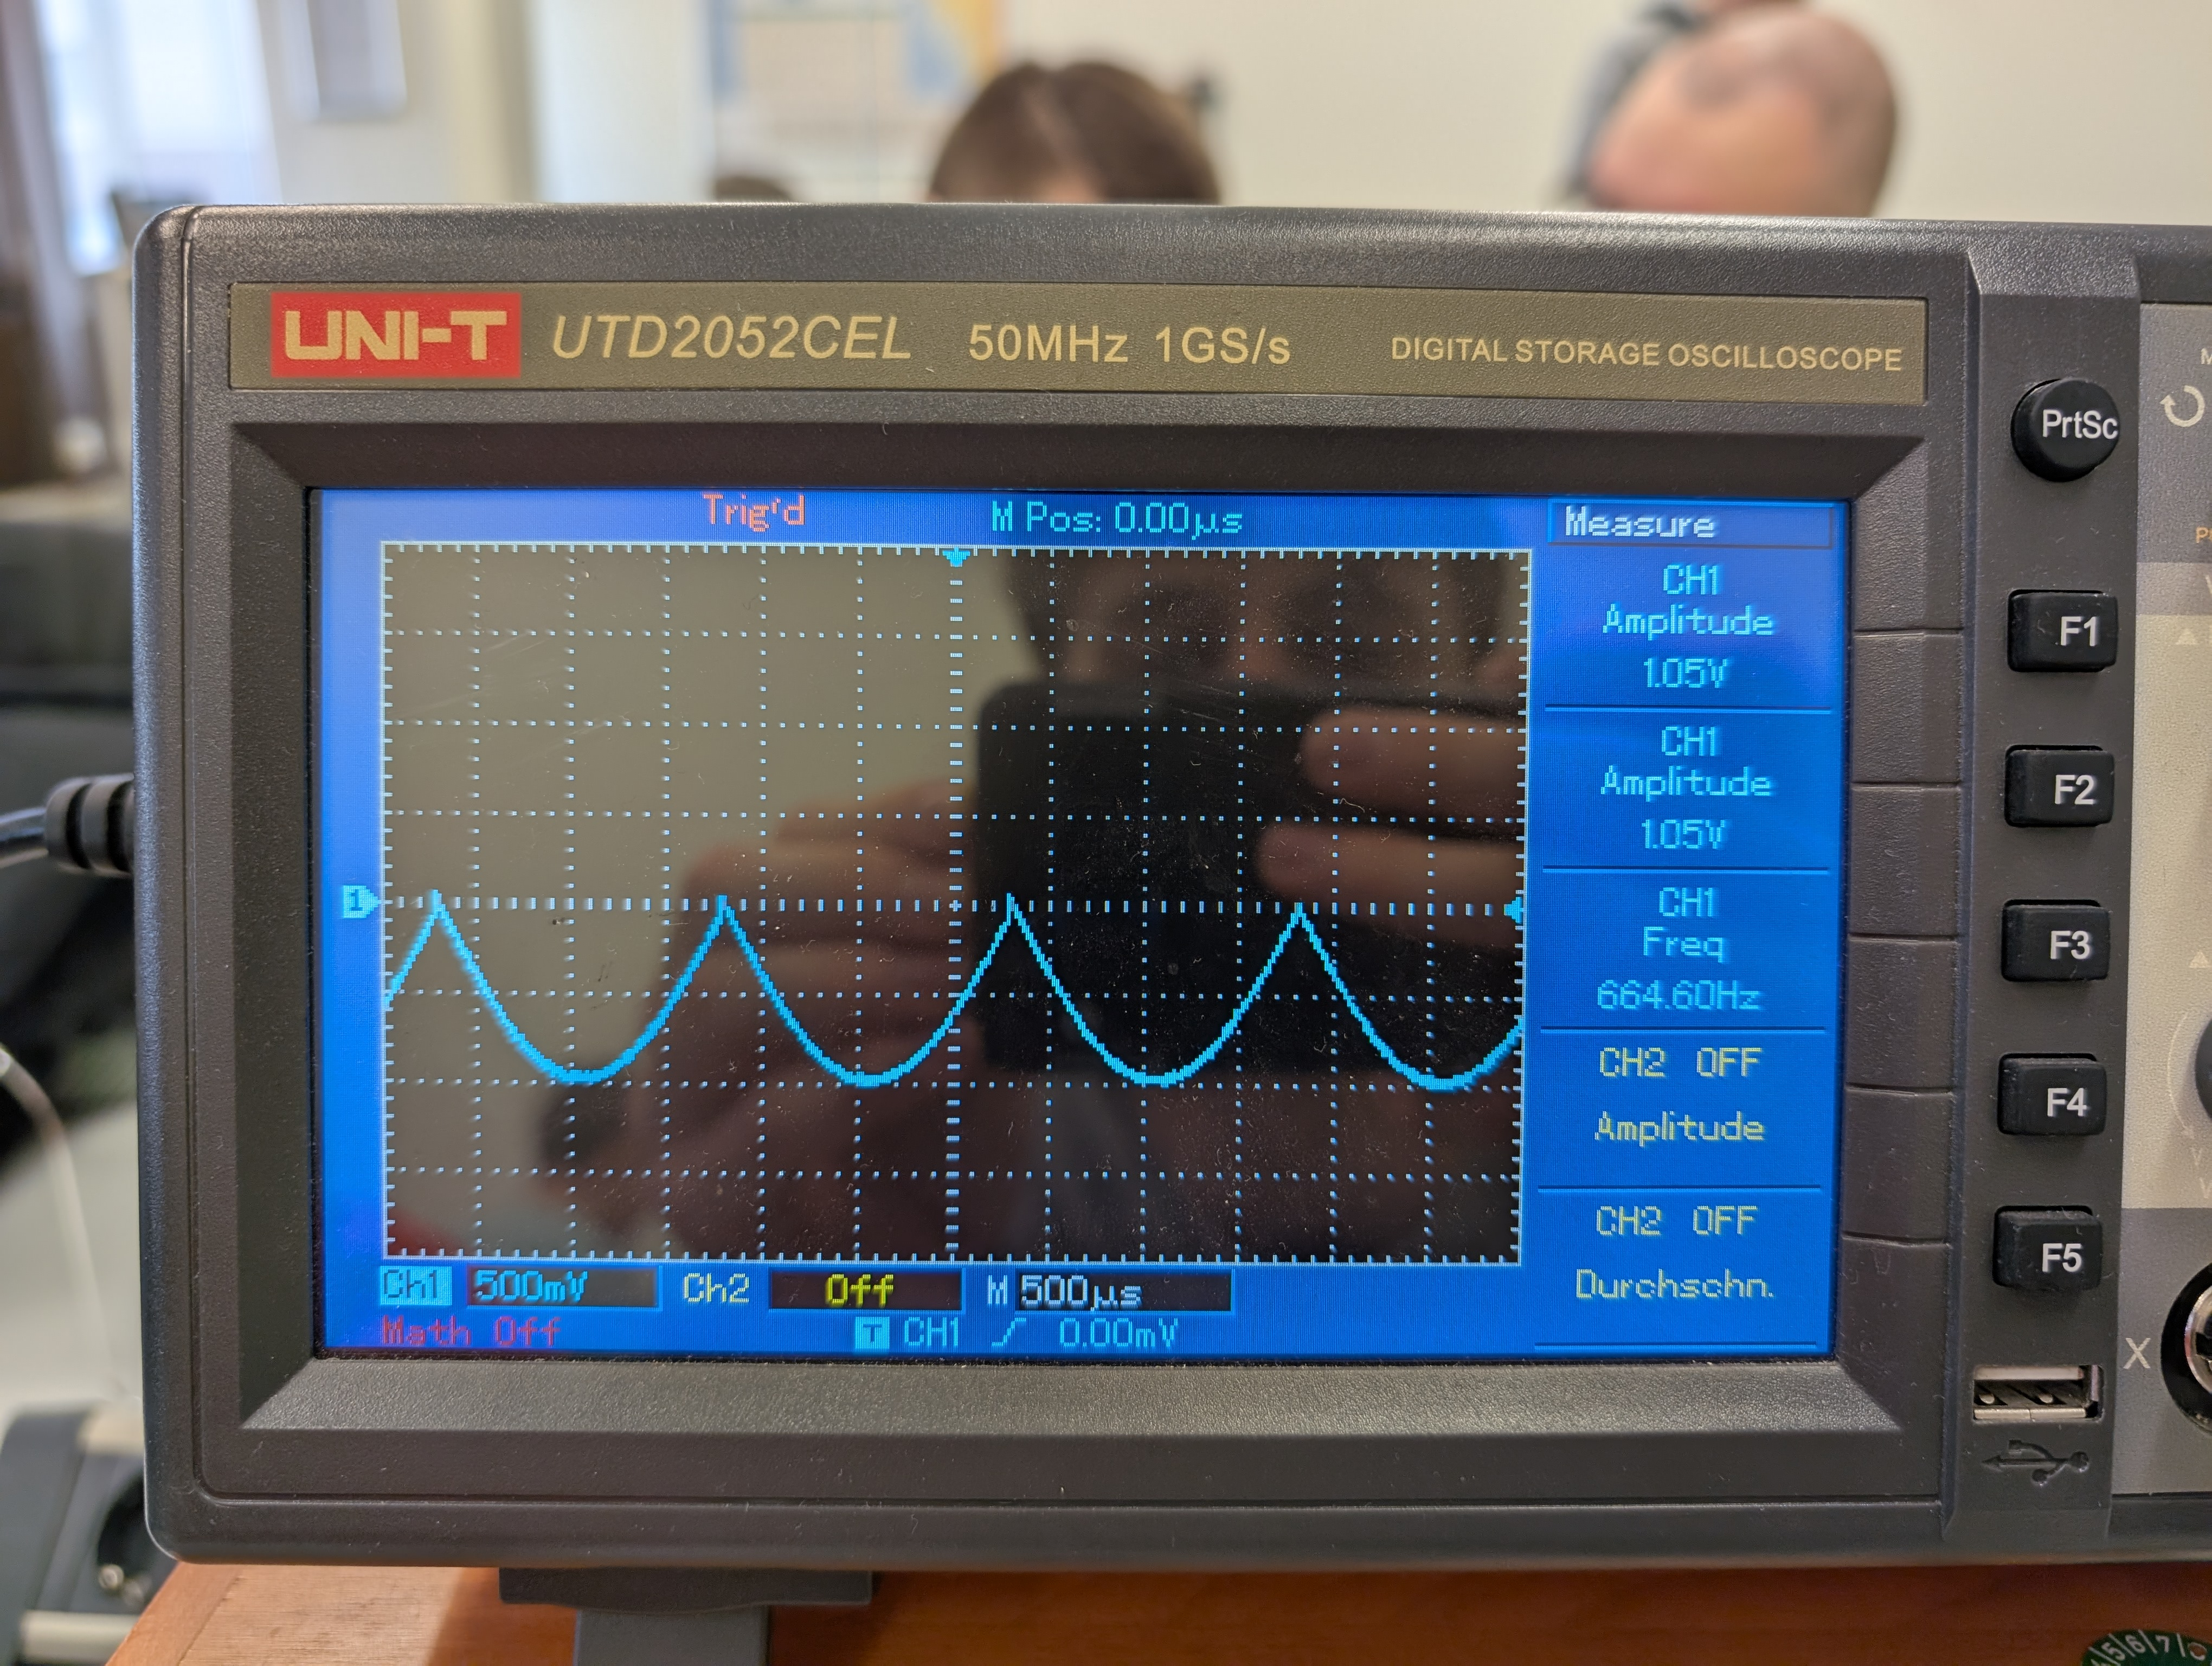
\includegraphics[width=0.5\textwidth]{"Bilder/270.jpg"}
\end{figure}
\begin{figure}
    \caption{Spannung bei 360$\unit{\degree}$}
    \label{fig:12}
    \centering
    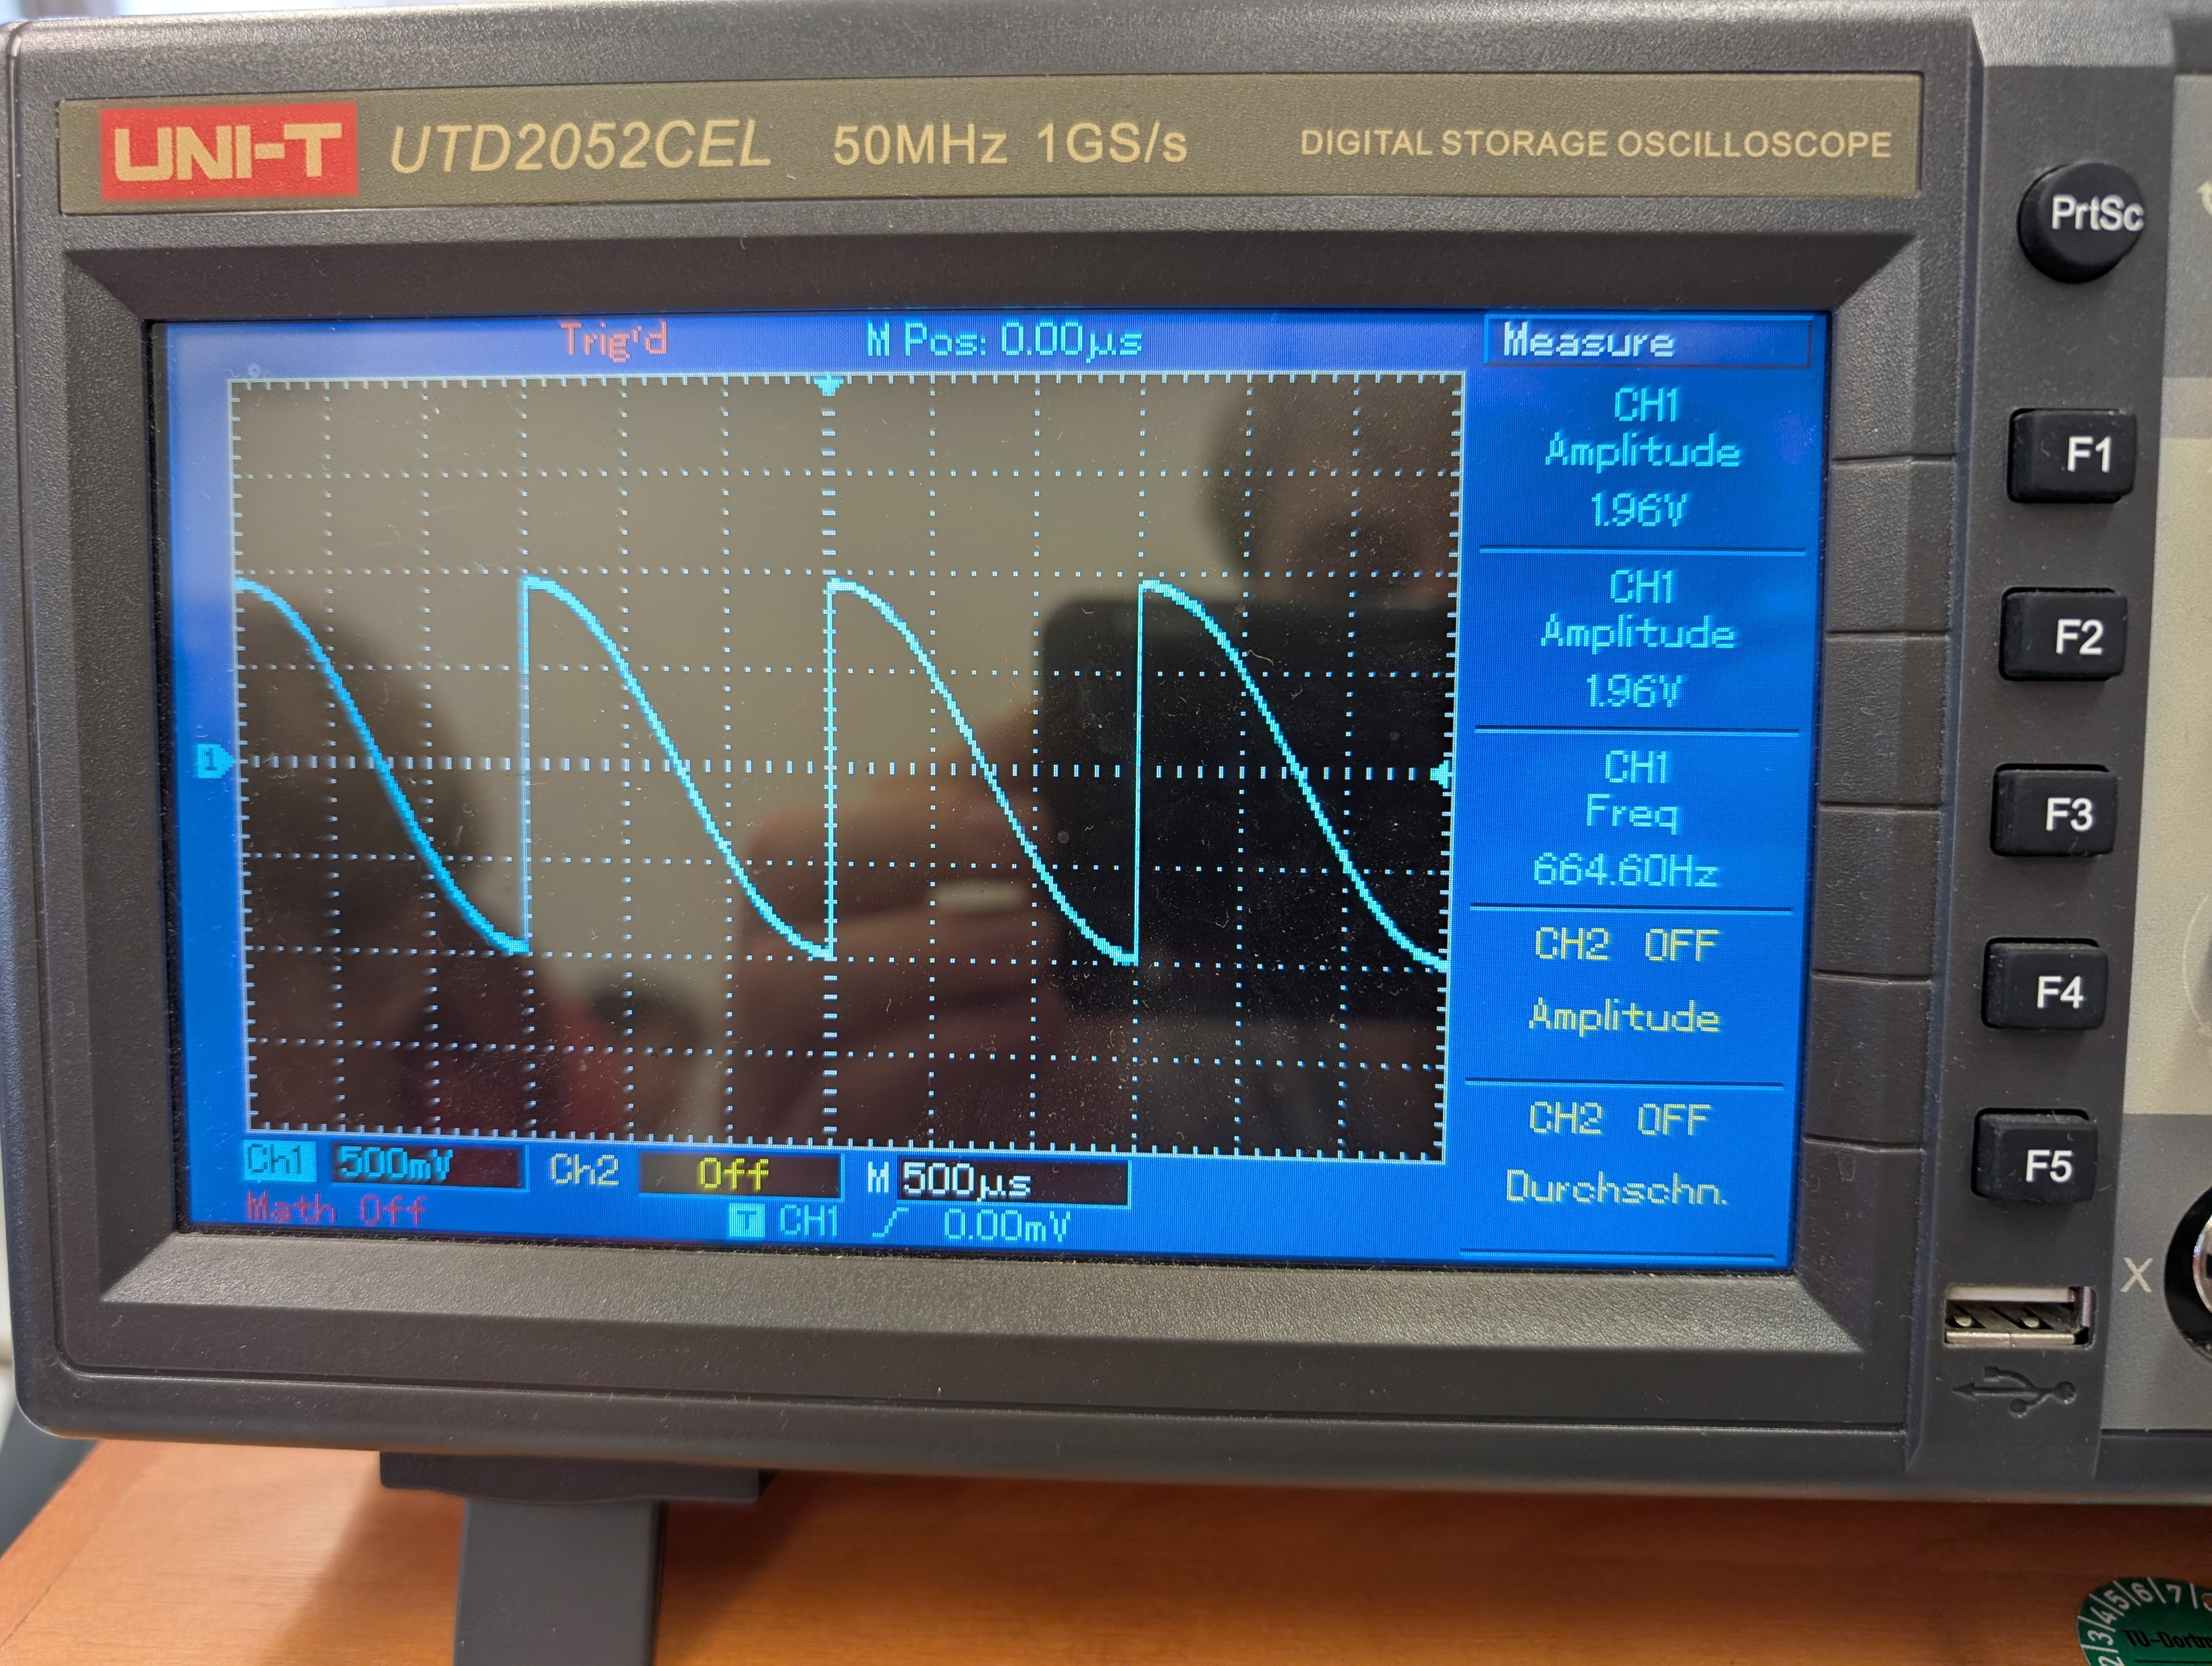
\includegraphics[width=0.5\textwidth]{"Bilder/360.jpg"}
\end{figure}

Um die Parameter wieder auf die Ausgangsspannung zurückzuführen wird \autoref{eqn:e4} nach der 
Amplitude der Eingangsspannung $U_0$ umgestellt.
\begin{equation}
    U_0 = U_{\text{out}} \cdot \frac{\pi}{2} 
\end{equation}







%Intensität/Abstand
\subsection{Verifizierung der Funktionsweise des Lock in Verstärkers Mit einer Leuchtdiode}
\begin{table}[H]
    \centering
    \caption{Lichtintensität in Abhängigkeit des Abstandes des Detektors zur Leuchtdiode}
    \label{tab:11}
    \begin{tblr}{
        colspec = {S S | S S},
        row{1} = {guard, mode=math},}
           \toprule
            \text{Phase} \left(\unit{\degree}\right) & U \left(\unit{\volt}\right) & \text{Phase} \left(\unit{\degree}\right) & U \left(\unit{\volt}\right)\\
           \midrule
           4.5   &  7   & 15     & 2    \\              
           5     &  7   & 15.5   & 1.5  \\    
           5.5   &  7   & 16     & 1.5  \\    
           6     &  6   & 16.5   & 1.5  \\    
           6.5   &  5   & 17     & 1.5  \\    
           7     &  5   & 17.5   & 1.5  \\    
           7.5   &  4.5 & 18     & 1.5  \\    
           8     &  4   & 18.5   & 1.5  \\    
           8.5   &  4   & 19     & 1    \\
           9     &  3.5 & 19.5   & 1    \\
           9.5   &  3.5 & 20     & 1    \\
           10    &  3   & 20.5   & 1    \\
           10.5  &  3   & 21     & 1    \\
           11    &  3   & 21.5   & 1    \\    
           11.5  &  2.5 & 22     & 1    \\
           12    &  2.5 & 22.5   & 1    \\
           12.5  &  2.5 & 23     & 1    \\
           13    &  2.5 & 23.5   & 1    \\
           13.5  &  2   & 24     & 0.5  \\    
           14    &  2   & 24.5   & 0.5  \\    
           14.5  &  2   & 25     & 0.5  \\    
           14.5  &  2   & 43     & 0    \\
            \bottomrule
    \end{tblr}
\end{table}
\begin{figure}[H]
    \caption{}
    \label{fig:11}
    \centering
    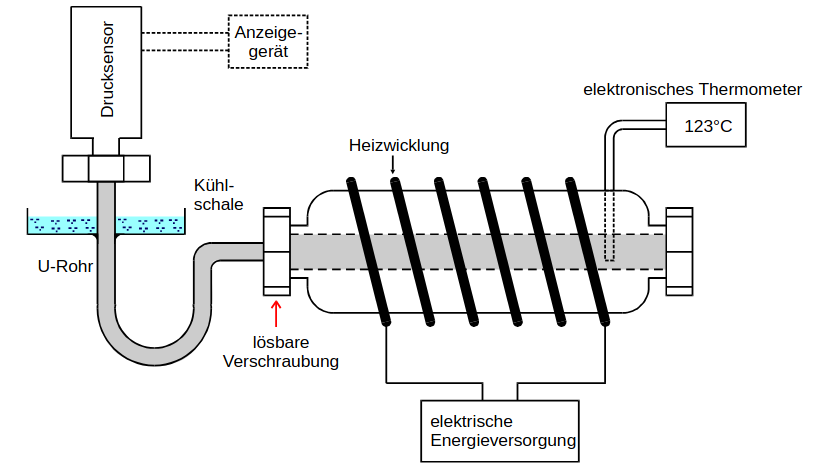
\includegraphics{"build/teil2.pdf"}
\end{figure}
In \autoref{tab:11} ist die Intensität des Lichts, welches von der Leuchtdiode ausgesendet wird 
zusammen mit dem jewailigen Abstand des Detektors zur Leuchdiode aufgetragen. In \autoref{fig:11}
ist die Intensität als Funktion des Abstandes geplottet und durch eine Ausgleichsrechnung 
durch Eine Funktion der Form 
\begin{equation}
    \symbf{I}\left(r\right) = a \cdot \frac{1}{x^b} + c
\end{equation}
genähert.
Die Ausgleichsparameter $a, b, c$ der Funktion lauten
\begin{align*}
    a = & \qty{31(11)}{\watt\centi\meter\squared}   \\
    b = & \qty{0.80(0.32)}{}     \\
    c = & \qty{-1.7(1.8)}{\watt}       
\end{align*}
Eigentlich sollte hier eine $\frac{1}{x^2}$ Abhängigkeit rauskommen, da diese nicht einmal 
näherungsweise im Fehlerbereich des Parameters b liegt, lässt dies auf grobe Ungenauigkeiten
im Experiment hindeuten.

\label{sec:Auswertung}
